\chapter{Plasma Models}

	\section{\texttt{spicedmodel}: The Scalable Plasma Ion Composition and Electron Density Model}



	\section{\texttt{spiced}}

	\section{\texttt{HermeanFLRModel}: Model of Mercury's dayside plasma mass density}

		GitHub: \href{https://github.com/mattkjames7/HermeanFLRModel.git}{https://github.com/mattkjames7/HermeanFLRModel.git}

		Estimate the dayside plasma mass density in Mercury's magnetosphere using the field line resonance (FLR) based model from \citet{James2019}.

		\subsection{Installation}

			This hasn't been placed on PyPI, so either download fromt he GitHub page and install using \texttt{pip}, or clone and build the package:
			\begin{minted}{bash}
#if you download the package
pip3 install HermeanFLRModel-x.y.z-py3-none-any.whl --user

#or clone, build and install
git clone https://github.com/mattkjames7/HermeanFLRModel.git
cd HermeanFLRModel
python3 setup.py bdist_wheel
pip3 install dist/HermeanFLRModel-x.y.z-py3-none-any.whl --user
			\end{minted}
			where \texttt{x.y.z} should be replaced with the current version number.

		\subsection{Usage}

			Import the module and create an instance of the \texttt{Model} object:
			\begin{minted}{python}
import HermeanFLRModel as hflr

model = hflr.Model(Alpha,Coord='MSM')
			\end{minted}
			where \texttt{Alpha} is the power law index which should be an integer from 0 to 6, and \texttt{Coord} sets the coordinate system to use (either MSM or MSO).

			Use the \texttt{model.Calc()} member function to work out densities:
			\begin{minted}{python}
#create input coordinate(s)
x = np.zeros(6)
y = np.array([1.0,1.2,1.4,1.6,1.8,2.0])
z = np.zeros(6)

#call model Calc() function
rho = model.Calc(x,y,z)
			\end{minted}

			Or produce a plot of the plasma mass denity for a slice through the magnetosphere, e.g.:
			\begin{minted}{python}
#select magnetic local time and alpha
MLT = 6.0
Alpha = 3.0

#plot it
ax = hflr.PlotModelSlice(MLT,Alpha)
			\end{minted}
			which should produce something like figure \ref{FigHFLR}.

			\begin{figure}
				\begin{center}
					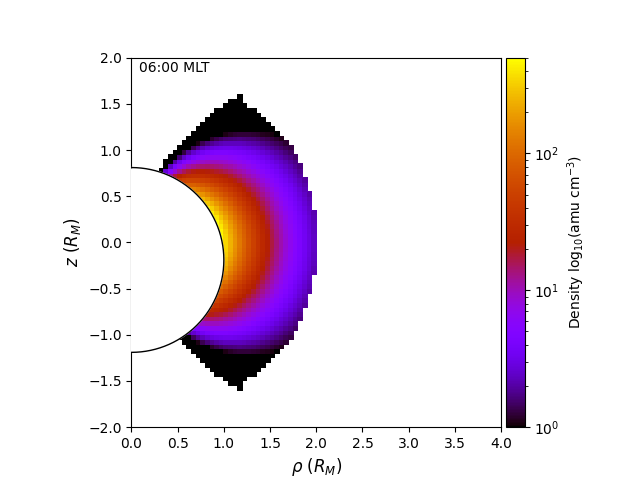
\includegraphics[width=0.8\textwidth]{figures/ch2_hflr.png}
				\end{center}
				\caption{Plasma mass density at 6:00 MLT. \label{FigHFLR}}
			\end{figure}



	\section{\texttt{PyGCPM}: Wrapper for the Global Core Plasma Model}
	
		GitHub: \href{https://github.com/mattkjames7/PyGCPM.git}{https://github.com/mattkjames7/PyGCPM.git}

		This is a Python wrapper for the Global Core Plasma Model (\citet{Gallagher2000}, \href{https://plasmasphere.nasa.gov/models/}{code found here})

		\subsection{Installation}

			This module exists on PyPI, so can be installed using \texttt{pip}:
			\begin{minted}{bash}
pip3 install PyGCPM --user
			\end{minted}

		\subsection{Usage}

			There are three functions:
			\begin{enumerate}
				\item \texttt{PyGCPM.GCPM()}: provides particle densities at positions defined in SM coordinates.
				\item \texttt{PyGCPM.PlotEqSlice()} : plots the density of a species in the equatorial plane.
				\item \texttt{PyGCPM.PlotMLTSlice()} : plots the density of a particle species in 
			\end{enumerate}

			Firstly, get some densities at some positions in SM coordinates, units of $R_E$:
			\begin{minted}{python}
import PyGCPM
ne,nH,nHe,nO = PyGCPM.GCPM(x,y,z,Date,ut,Kp=Kp,Verbose=Verbose)
			\end{minted}
			where \texttt{Date} is the date in the format yyyymmdd, \texttt{ut} is the time in hours, \texttt{Kp} is the Kp index and \texttt{Verbose=True} would display progress. The outputs of this function \texttt{ne}, \texttt{nH}, \texttt{nHe} and \texttt{nO} are the densities of electrons, protons, helium ions and oxygen ions, respectively.

			We can plot the density of a particle species in the equatorial plane:
			\begin{minted}{python}
PyGCPM.PlotEqSlice(20010902,12.0,Parameter='ne')
			\end{minted}
			which should produce the plot in figure \ref{FigPyGCPMEq}.

			\begin{figure}
				\begin{center}
					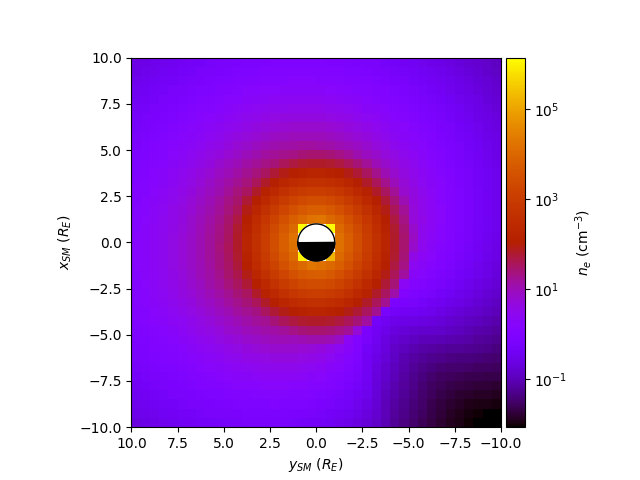
\includegraphics[width=0.8\textwidth]{figures/ch2_pygcpm_equator.png}
				\end{center}
				\caption{Equatorial electon density. \label{FigPyGCPMEq}}
			\end{figure}

			We can also plot the density of a particle species in a slice of MLT:
			\begin{minted}{python}
PyGCPM.PlotMLTSlice(8.0,20010902,12.0,Parameter='ne')
			\end{minted}
			which should produce the plot in figure \ref{FigPyGCPMMLT}.

			\begin{figure}
				\begin{center}
					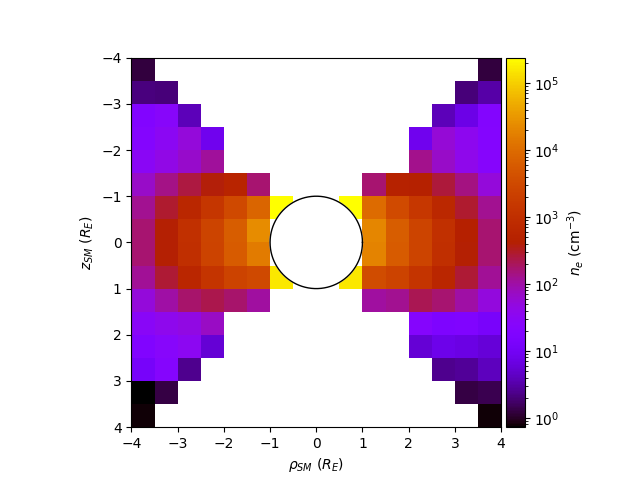
\includegraphics[width=0.8\textwidth]{figures/ch2_pygcpm_mlt.png}
				\end{center}
				\caption{MLT slice of electon density. \label{FigPyGCPMMLT}}
			\end{figure}